\usetikzlibrary{patterns}

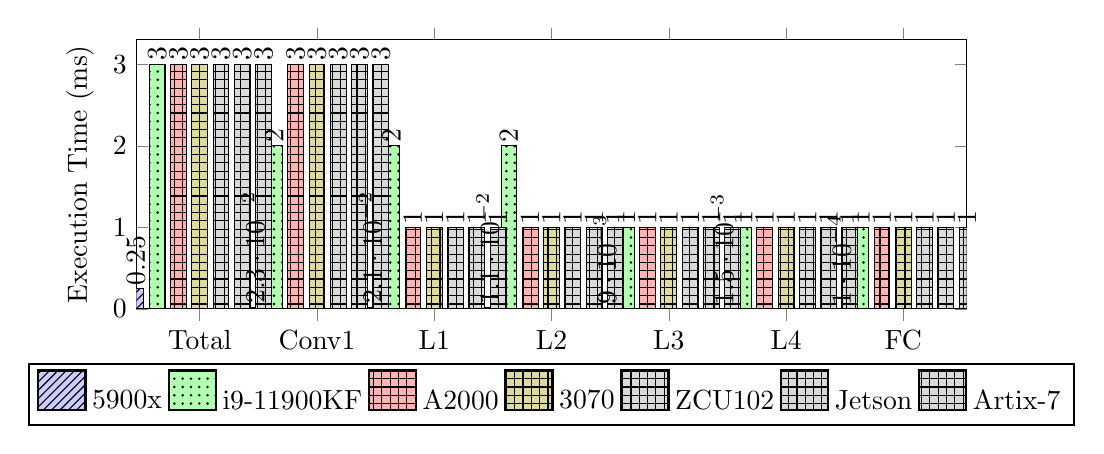
\begin{tikzpicture}
  \begin{axis}[                  
  ybar,  
  ymin=0, 
  width=\textwidth,                                
  height=5cm,                                
  legend image code/.code={                                                        \draw[#1, draw=none] (0cm,-0.1cm) rectangle (0.6cm,0.4cm);
  },
  legend style={
    at={(0.5,-0.20)},
    anchor=north,
    legend columns=-1,
    draw=black,
    fill=white,
    thick
  },
  ylabel={Execution Time (ms)},
  symbolic x coords={Total,Conv1,L1,L2,L3,L4,FC},
  xtick=data,
  nodes near coords,
  nodes near coords style={
    anchor=west,
    rotate=90,
    inner xsep=1pt
  },
  enlarge x limits=0.09,
  bar width=0.2cm,
  ]
  \addplot[pattern=north west lines,pattern color=black, fill=blue!20, postaction={pattern=north east lines}] coordinates {(Total, 0.25)(Conv1, 0.023)(L1, 0.021)(L2, 0.011)(L3, 0.009)(L4, 0.0015)(FC, 0.0001)};
  \addplot[pattern=north east lines,pattern color=black,fill=green!30, postaction={pattern=dots}] coordinates {(Total, 3)(Conv1, 2)(L1, 2)(L2, 2)(L3, 1)(L4, 1)(FC, 1)};
  \addplot[pattern=dots,pattern color=black,fill=red!30, postaction={pattern=grid}] coordinates {(Total, 3) (Conv1, 3)(L1, 1)(L2, 1)(L3, 1)(L4, 1)(FC, 1)};
 \addplot[pattern=crosshatch,pattern color=black,fill=olive!30, postaction={pattern=grid}] coordinates {(Total, 3) (Conv1, 3)(L1, 1)(L2, 1)(L3, 1)(L4, 1)(FC, 1)};
  \addplot[pattern=vertical lines,pattern color=black,fill=gray!30, postaction={pattern=grid}] coordinates {(Total, 3) (Conv1, 3)(L1, 1)(L2, 1)(L3, 1)(L4, 1)(FC, 1)};
\addplot[pattern=vertical lines,pattern color=black,fill=gray!30, postaction={pattern=grid}] coordinates {(Total, 3) (Conv1, 3)(L1, 1)(L2, 1)(L3, 1)(L4, 1)(FC, 1)};
\addplot[pattern=vertical lines,pattern color=black,fill=gray!30, postaction={pattern=grid}] coordinates {(Total, 3) (Conv1, 3)(L1, 1)(L2, 1)(L3, 1)(L4, 1)(FC, 1)};
  
  \legend{5900x,i9-11900KF,A2000,3070,ZCU102,Jetson,Artix-7}
  \end{axis}
\end{tikzpicture}

